\documentclass[../report.tex]{subfiles}
\begin{document}	
	
\chapter{State of the art}
The most interesting aspect of fabricating optical waveguides from silicon is based on low primary cost of material, the mature and evolved manufacturing techniques owing to decades of research and the potential to develop monolithic \gls{ic} using the same substrate.

	\section{Theoretical background of SOI waveguide}
Although silicon is the optimal material for electronics, only recently silicon is being considered as a practical option for \gls{oeic} solutions. Silicon has many properties conducive to fiber optics. The band gap of silicon ($\sim$\SI{1.1}{\electronvolt}) is such that the material is transparent to wavelengths commonly used for optical transport ($\sim$\SI{1.3}{\micro\metre}-\SI{1.6}{\micro\metre}). One can use standard \gls{cmos} processing techniques to sculpt optical waveguides onto the silicon surface. Similar to an optical fiber, these optical waveguides can be used to confine and direct light as it passes through the silicon \cite{reed_silicon_2004}. Due to the wavelengths typically used for optical transport and silicon’s high index of refraction, the feature sizes needed for processing these silicon waveguides are on the order of \SI{0.5}{\micro\metre}-\SI{1}{\micro\metre}. The lithography requirements needed to process waveguides with these sizes exist today. If we push forward to leading-edge research currently under way in the area of \gls{pbg} devices, today’s state-of-the-art \SI{90}{\nano\metre} fabrication facilities should meet the technical requirements needed for processing \gls{pbg} devices. What this says is that we may already have all or most of the processing technologies needed to produce silicon-based photonic devices for the next decade. In addition, the same carriers used for the basic functionality of the transistor (i.e. electrons and holes) can be used to modulate the phase of light passing through silicon waveguides and thus produce ‘active’ rather than passive photonic devices. Finally, if all this remains \gls{cmos}-compatible, it could be possible to process transistors alongside photonic devices, the combination of which could bring new levels of performance, functionality, power and size reduction, all at a lower cost.
		
		\subsection{Maxwell's equations}
Light is high frequency \gls{em} phenomenon having wave-particle duality. Visible light, ultraviolet light, and infrared light are all electromagnetic waves of differing frequency. 
\begin{figure}[h]
	\centering
	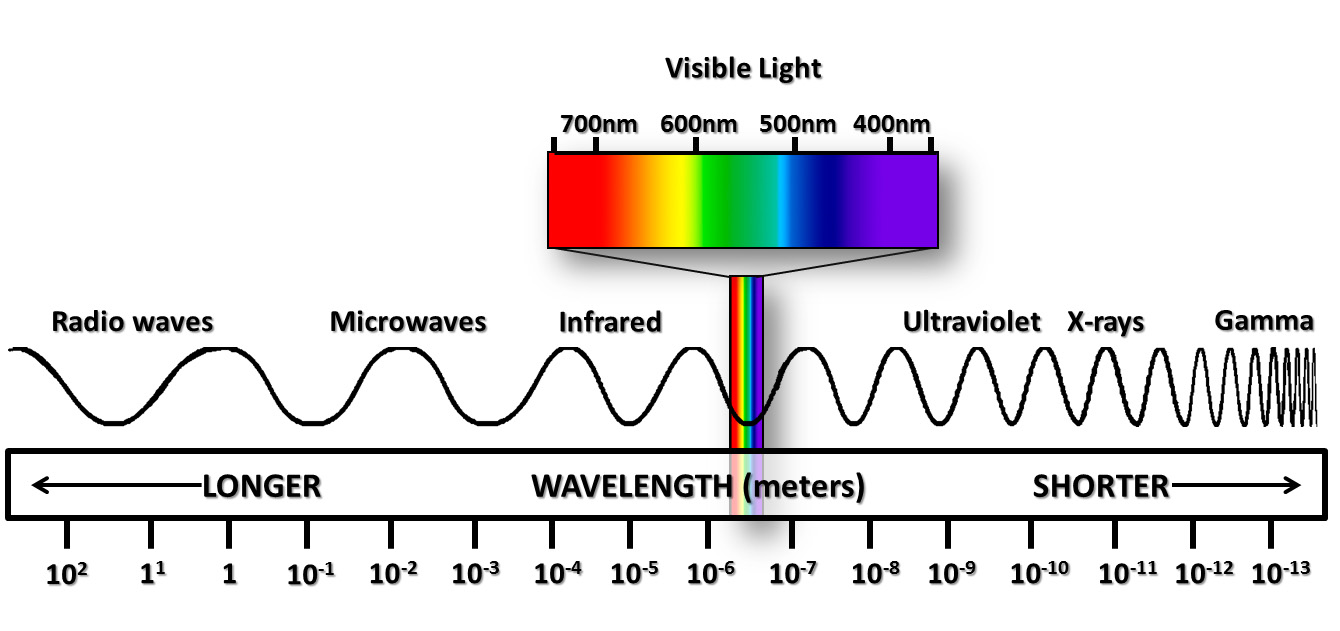
\includegraphics[width=0.75\textwidth]{2-light-spectrum}
	\caption{The \gls{em} wave spectrum}
	\label{fig:2_light_spectrum}
\end{figure}
James Clerk Maxwell discovered that he could combine four simple equations, which had been previously discovered, along with a slight modification to describe self-propagating waves of oscillating electric and magnetic fields \cite{waveparticle_2016}. The understanding of propagating of light waves using Maxwell's equations in a dielectric medium, is the key to the construction of silicon waveguides. Maxwell’s equations relate the electric field $E$ (V/m), magnetic field $H$ (A/m), charge density $\rho$ (C/m3), and current density $J$ (A/cm2).
\begin{itemize}	
	\item \textbf{Maxwell's first equation (Gauss' Law)}: The net electric flux through any closed surface is equal to $\frac{1}{\epsilon_m}$ times the charge density within that closed surface.
	\begin{equation}\label{eq:max1_1}
	\nabla.E = \frac{\rho}{\epsilon_m}	
	\end{equation}
	where $\epsilon_m$ the permittivity of the medium, and del operator, $\nabla$, is given by:
	\begin{equation}\label{eq:max1_2}
	\nabla = \left(\frac{\partial i}{\partial x},\frac{\partial j}{\partial y},\frac{\partial k}{\partial z}\right)
	\end{equation}
	where i, j and k are unit vectors in the x, y and z directions respectively.
	
	\item \textbf{Maxwell's second equation (Gauss' Law for magnetic field)}: The net magnetic flux through a closed surface is always zero since magnetic monopoles do not exist.
	\begin{equation}\label{eq:max1_3}
	\nabla.H = 0	
	\end{equation}
	
	\item \textbf{Maxwell's third equation (Faraday's law)}: Induced electric field around a closed path is equal to the negative of the time rate of change of magnetic flux enclosed by the path.
	\begin{equation}\label{eq:max1_4}
	\nabla\times E = -\mu_m\frac{\partial H}{\partial t}
	\end{equation}
	where $\mu_m$ is the permeability of the medium.
	
	\item \textbf{Maxwell's fourth equation (Modification of Ampere's law)}:  The fourth equation states that magnetic fields can be generated in two ways: by electric current (this was the original "Ampere's law") and by changing electric fields (this was "Maxwell's addition") \cite{wiki_maxwells_2016}.
	\begin{equation}\label{eq:max1_5}
	\nabla\times H =  J + \epsilon_m\frac{\partial E}{\partial t}	
	\end{equation}	
\end{itemize}

All these equations combine into a simple wave equation after some mathematical calculations.
\begin{equation}\label{eq:wave_eq}
\nabla^2 E -  \mu_m\epsilon_m\frac{\partial^2 E}{\partial t^2} = \mu_m\frac{\partial J}{\partial t} + \frac{\nabla\rho}{\epsilon_m}	
\end{equation}
using the curl of curl identity operation given by: 
\begin{equation}\label{eq:curl_of_curl}
\nabla^2 E = \nabla(\nabla.E) - \nabla\times(\nabla\times E)
\end{equation}
A general solution to the equation \ref{eq:wave_eq} in free space, in absence of charge gives the following solution:
\begin{equation}\label{eq:wave_sol_electric}
E=E_{0}(x,y)e^{i\left(k_{0}z\pm \omega t\right)}
\end{equation}
where $z$ is direction of propagation of wave in Cartesian coordinates , phase ($\phi$) = $\left(k_{0}z\pm \omega t\right)$ and wave vector propagation constant ($k_0$) = $\dfrac {\partial \phi } {\partial t}$ = $\dfrac {2\pi } {\lambda }$, in the direction of propagation of the wave. It is worth mentioning that propagation constant in medium varies according to $n$, the \gls{ri} of the medium and is given by: 
\begin{equation}\label{eq:ri_med_val}
k = nk_0
\end{equation}
Similar calculations for the magnetic field, $H$ in free space yields, 		
\begin{equation}\label{eq:wave_sol_magnetic}
H=H_{0}(x,y)e^{i\left(k_{0}z\pm \omega t\right)}
\end{equation}

		\subsection{Eigenvalue and wave modes}
In general the electric field in the wave equation in \ref{eq:wave_sol_electric} can be written in its constituent parts in Cartesian coordinates as:
\begin{equation}\label{eq:e_field_cart_cord}
E=E_{x}i+E_{y}j+E_{j}k
\end{equation}
If the wave propagates towards z-direction through any waveguide medium and is a \gls{tem} wave front then we will have a constant electric field vector in the z-direction. In this case there will be different solutions for the propagation constant in x and y directions. Now for each solution we can also get certain discrete angles at which the electric field can travel through the medium, which infers that light can propagate only at certain discrete angles through any dielectric medium. Each allowed solution is referred to as the \textit{mode of propagation} and are basically the different eigenvalues of the propagation vector. In the Fig. \ref{fig:2_em_wave} the electric field and magnetic field propagate in directions perpendicular to each other. Moreover, the direction of propagation is also transverse to the \gls{em} field. Hence it is called \gls{tem} wave.
\begin{figure}[H]
	\centering
	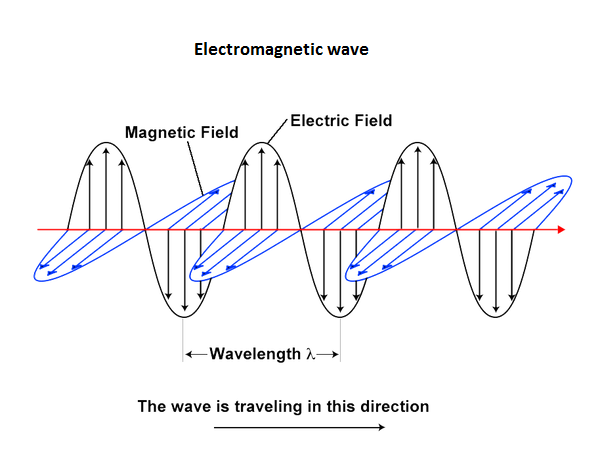
\includegraphics[width=0.75\textwidth]{2-em-wave}
	\caption{Propagation of \gls{em} wave}
	\label{fig:2_em_wave}
\end{figure}
\begin{figure}[H]
	\centering
	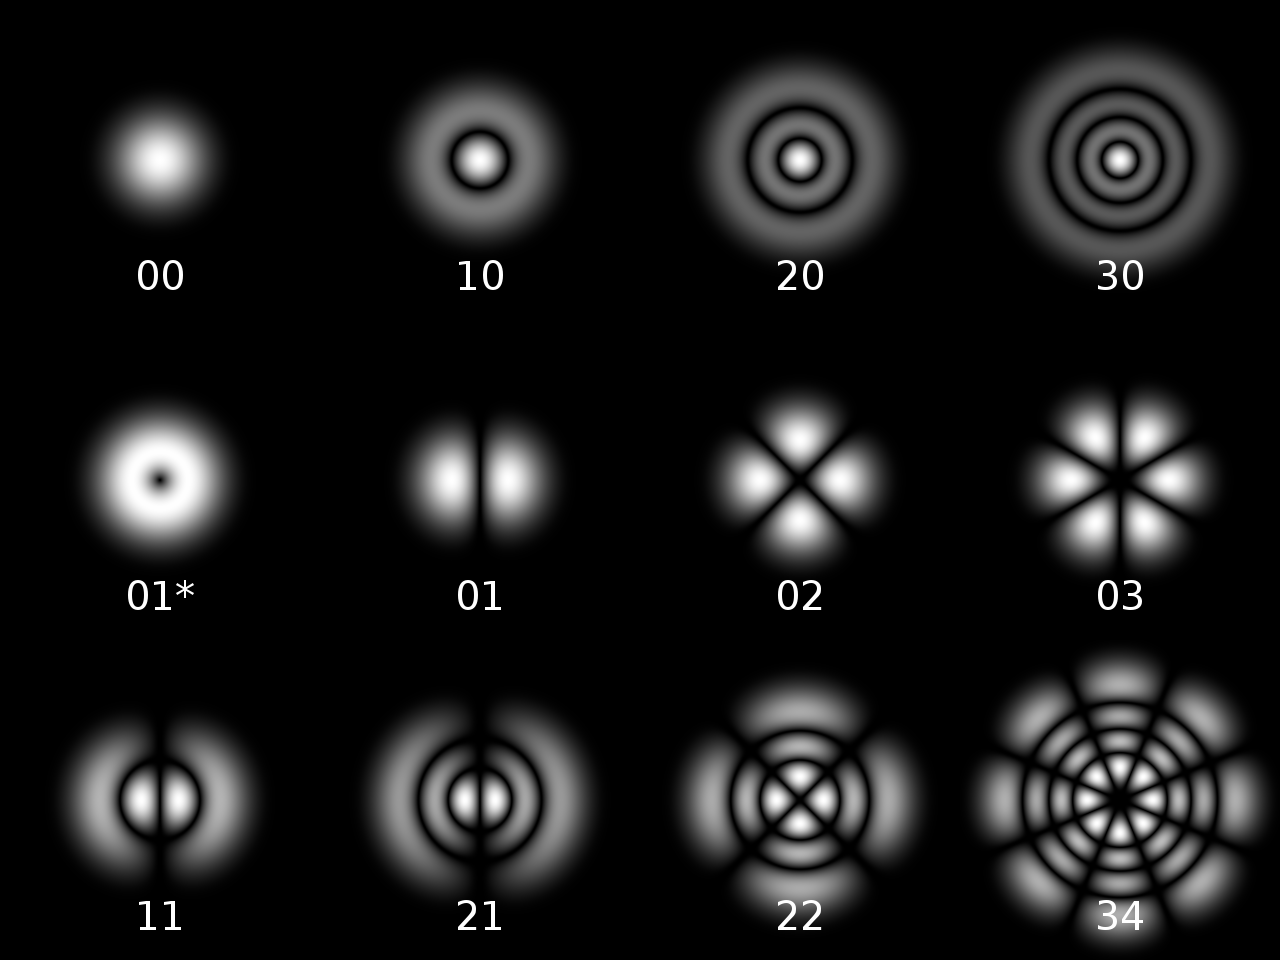
\includegraphics[width=0.75\textwidth]{2-modes}
	\caption{Propagation modes in optical fiber}
	\label{fig:2_modes}
\end{figure}
The eigenvalues provide the different acceptance angles at which light can be inserted into the waveguide resulting in different modes in the waveguide. Depending on various angles of incidence on the waveguide and the dimensions of the waveguide, various modes can be found which are basically the different eigenvalues of the wave solution \ref{eq:wave_sol_electric} and \ref{eq:wave_sol_magnetic}. For example, when light travels through optical fibers different modes can be visualized as follows in Fig. \ref{fig:2_modes}.
\todo{May be update the picture using CST}
		\subsection{Optical polarization and transverse modes}
Generally light in randomly polarized. Any kind of randomness is inefficient for data transmission. Optical fibers generally operate at \SI{1550}{\nano\metre} in fundamental \gls{te} or \gls{tm} mode. The ultimate goal of the on chip fabricated waveguide is to integrate with the currently deployed optical fiber network in a seamless manner. Hence, the waveguides must cater polarization into its design.  
\begin{figure}[h]
	\centering
	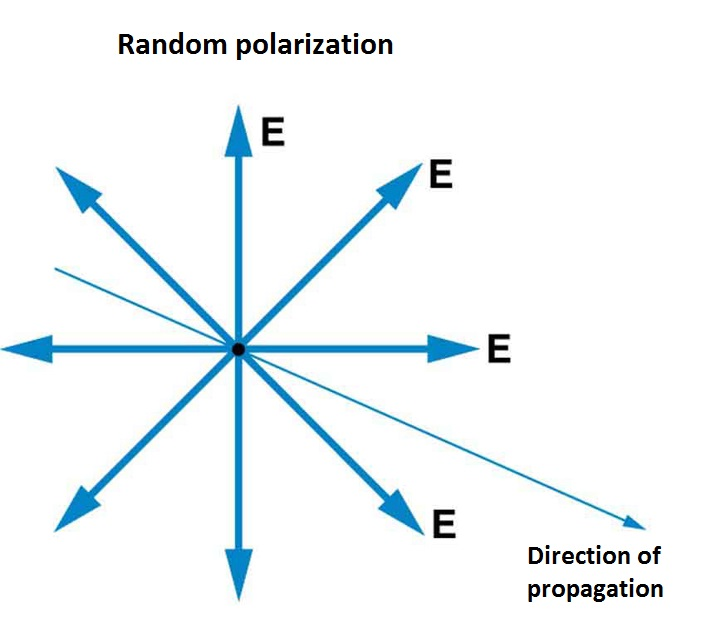
\includegraphics[width=0.75\textwidth]{2-random-pol}
	\caption{Random polarization of light}
	\label{fig:2_random_pol}
\end{figure}
\textit{Polarization} is the direction of the electric field associated with the propagating wave. However, the associated magnetic field is not always considered in the quantum domain for wave propagating at \SI{1550}{\nano\metre}. In the example in Fig. \ref{fig:2_em_wave} the wave is polarized since the electric field and magnetic field exist in one direction only. In a semiconductor optical waveguide light propagates in plane polarized modes and the plane in which light is polarized is either vertical or horizontal to the waveguide surface as shown in Fig. \ref{fig:2_te_tm_mode}. 
\begin{figure}[H]
	\centering
	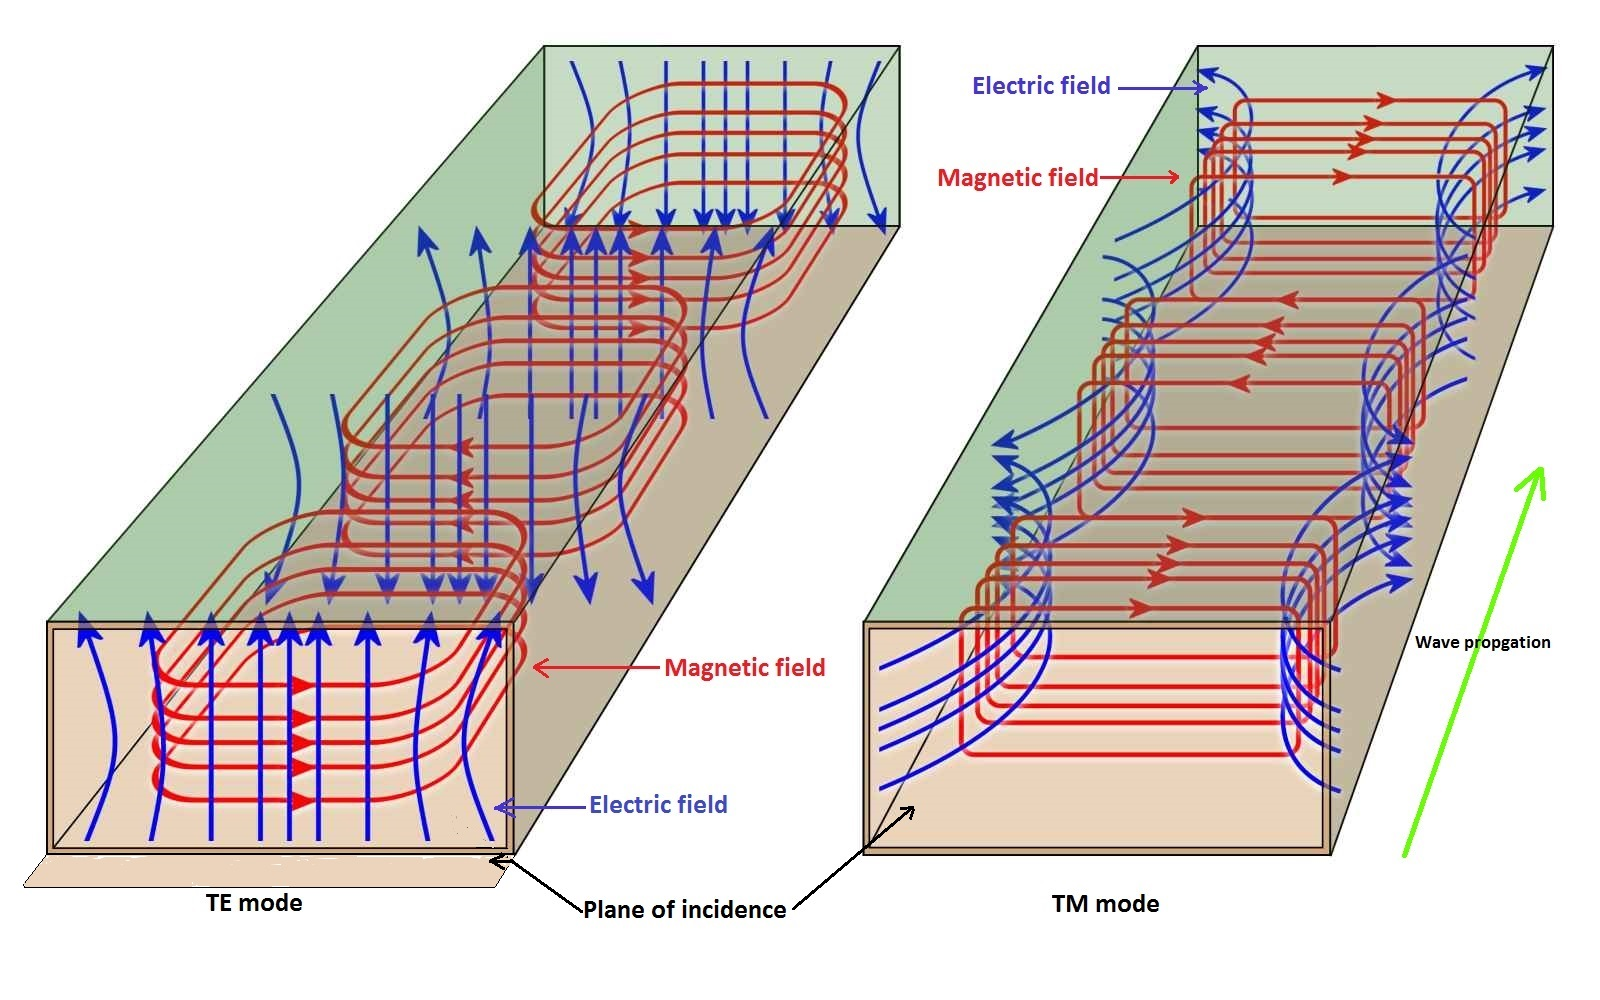
\includegraphics[width=0.75\textwidth]{2-te-tm-mode}
	\caption{\gls{te} and \gls{tm} modes in a waveguide}
	\label{fig:2_te_tm_mode}
\end{figure}			
			\subsubsection{TE mode}
\gls{te} mode is the fundamental mode in which electric field is perpendicular to the plane of incidence of light. As depicted in Fig. \ref{fig:2_te_tm_mode} it can be visualized that electric field lines shown by the blue lines are perpendicular to the plane of incidence in \gls{te} mode. The plane of incidence is the plane in which optical waves strike the surface of the waveguide.						
			\subsubsection{TM mode}
\gls{tm} mode is the fundamental mode in which magnetic field is perpendicular to the plane of incidence of light. As shown in Fig. \ref{fig:2_te_tm_mode} it can be visualized that magnetic field shown by the red lines are perpendicular to the plane of incidence in \gls{tm} mode.			
		\subsection{Optical waveguides}
			
			\subsubsection{Planar waveguides}
			
			\subsubsection{Rib waveguides}			
		
		\subsection{Jones vector}
		
		\subsection{Transfer matrix (S-matrix)}
		
		\subsection{Poincaré sphere}
		
		\subsection{Polarization in optical waveguides}
		
	\section{Theoretical background of MEMS}
	
		\subsection{Overview}
		
		\subsection{Actuation principle}
			
	\section{Polarization rotator}
	
		\subsection{Passive polarization rotator}
	
		\subsection{Active polarization rotator}
\end{document}
